\chapter{Experiment 2: Effectiveness of Distractors}
This chapter consists of the Method, Results and Discussion components for Experiment 2. The experiment itself focuses on various effectiveness metrics for the developed redirected walking solution. 

\section{Method}
As part of developing the extension to the redirected walking toolkit, one of the implemented components was the AC2F algorithm. Since AC2F makes use of more predictive information compared to S2C, it would be interesting to see whether this provides a more effective solution when using distractors. As such, this experiment compares two different conditions. The first makes use of S2C only throughout an entire playthrough of Ensemble Retriever while the other uses S2C during walking and AC2F during the standing distractor battles. The redirection gains employed in this experiment are derived from the estimated thresholds in Chapter~\ref{chap:ex1}. 

This section consists of the related methods that have been used to measure and test the effectiveness of employing AC2F when using distractors. 

\subsection{Hypotheses}
In order to test effectiveness, it is first necessary to operationalise the term. For this experiment there are two primary types of effectiveness that have been focused on. The first of these is Azmandian et al.'s relative effectiveness~\cite{azmandian2015physical}. Relative effectiveness provides a measurement of redirection effectiveness through the number of resets that happen throughout one condition compared to another. It is defined with the following formula:
$$
RelativeEffectiveness_{Algorithm} = \frac{ResetCount_{ControlCondition} - ResetCount_{ExperimentalCondition}}{ResetCount_{ControlCondition}}
$$
This results in the percentage difference of the experimental condition compared to the control counterpart. 

The second effectiveness metric that this experiment focuses on is effectiveness in terms of the time in seconds it takes for the user's future path to be aligned to the centre of the room. The distractor solution is in general agnostic to the redirection algorithm that is employed and simply disables any redirection whenever the future virtual path is aligned with the physical centre. This means that it is simple to compare S2C and AC2F for this effectiveness metric.

Given the two effectiveness metrics that the experiment focuses on, two null hypotheses have been established:
\begin{description}
  \item[$H_{0_1}$:] Employing S2C+AC2F in Ensemble Retriever does not provide significantly better relative effectiveness compared to S2C only. 
  \item[$H_{0_2}$:] Employing S2C+AC2F in Ensemble Retriever does not result in significantly lower time needed to align the user's future path towards the centre of the room compared to S2C only.
\end{description}


\subsection{Data Collection}
Experiment 2 employs a similar data collection procedure to Experiment 1. It records data every frame that Ensemble Retriever is running and focuses on recording data that is relevant to the two established null hypotheses. Some of these include data on when and how many resets that have been triggered, how much time it takes to be aligned with the centre of the room and the time it takes to defeat a distractor. A full list with descriptions for each piece of recorded data can be found in Section~\ref{sec:ex2dataformat}. 

\subsection{Data Post Processing}\label{sec:ex2postprocessing}
One problem that can affect the results for testing both hypotheses is what could be considered as ''unintentional resets''. These are resets that can happen during distractor battles in two different ways:
\begin{enumerate}
    \item If the user is walking fast enough, the buffer between a distractor triggering and a reset triggering might be too small, so by the time the user stops they have reached the boundary for triggering a reset. This means that the user is almost instantly aligned to the physical centre. 
    \item If the user moves around a lot during battles they risk triggering a reset since they already are close to the physical bounds while fighting. 
\end{enumerate}

Both of these cases could be considered as resets that are unintentional and would skew the results. In terms of frequency, it is the first of these cases that was the most apparent from observation of participants as they played. As such, a data processing step was conducted to attempt removing as many of these unintentional resets as possible. 

In terms of removing unintentional resets, there are two potential options. The first of these is to simply not include any resets that happen during battles with distractors. This is the simple solution, but may not end up including legitimate resets that happen between the start and end of a distractor's death animation. A distractor is considered as inactive after this death animation has finished. There are cases where participants start to walk right as a distractor's death animation starts which means that this method is not ideal as it may miss resets that happen in this time range. 

The second option is to discard any resets that happen within a given time buffer from when a distractor spawns. This is harder from a post processing perspective, but should provide more accurate results. This means that it can include the legitimate resets that may happen at the end of a distractor's life cycle while minimising the amount of unintentional resets. 
In order to decide the length of this time buffer it is first necessary to understand the minimum time a distractor battle has taken. For the recorded data in this experiment, the minimum time was \textasciitilde18.23 seconds. Since this time is recorded at the end of a distractor's death animation it is necessary to provide some buffer so that legitimate resets can be identified.

Given the minimum distractor duration of 18.28 seconds and the need for some buffer, the post processing uses a time of 10 seconds. This means that any resets that happened within the first 10 seconds of a distractor spawning become discarded from the analysis. A walkthrough for the entire post processing procedure can be found in Section~\ref{sec:ex2postprocessingdetails}.

\subsection{Sample}
* Intro
* Participants from experiment 1 were allowed to take part in experiment 2 as well if they wanted to

\subsubsection{Sampling Procedure}

The sampling procedure for Experiment 2 was the same as with Experiment 1. It consisted of advertisement by supervisors during lectures, information posters that were  placed around campus, advertisement on the local NTNU Discord server and general convenience sampling. Participants were once again compensated with some chocolate for their time. In total 15 participants signed up for Experiment 2, albeit only 13 of these showed up. These 13 were randomly distributed between the two conditions using the same Mersenne Twister library~\cite{MersenneTwisterLibraryLink} that previously has been mentioned throughout Chapter~\ref{chap:implementation}. This resulted in 7 participants for the control/S2C only condition and 6 in the experimental/S2C+AC2F condition. 

\subsubsection{Sample Demographics}

* Primarily within the age range of 18-24
* All males
* One had to remove optical corrections
* 11/13 had previous experience with redirected walking experiments
* Spread of VR Experience: Figure~\ref{fig:ex2PriorVRExperience}

\begin{figure}[tbph]
    \centering
    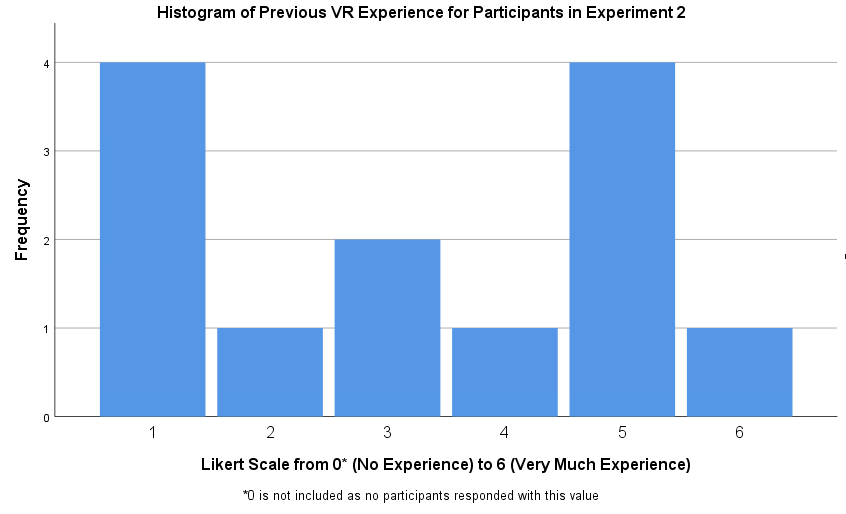
\includegraphics[width=0.75\textwidth]{figures/graphs/PriorVRExperienceExperiment2.png}
    \caption[Histogram on Prior VR Experience of Participants in Experiment 2]{This histogram shows the frequencies of what values participants provided in the demographics questionnaire of experiment 2 in terms of prior VR experience.}
    \label{fig:ex2PriorVRExperience}
\end{figure}

\subsubsection{Information and Consent}
* Brief information summary
* Specific details on what information participants were given can be found in Section~\ref{sec:ex2information}.
* Consent sheets can be found in Appendix~\ref{app:informationconsent}.


\subsubsection{Miscellaneous Information and Issues}
Section~\ref{sec:ex2environmentchanges}.
   * Participant 1 and 2 had some calibration problems
      * Participant 1 had 1 reset that should have triggered
      * Participant 2 had 2 resets that should have triggered
      * Eventually if I am unsure, I might have to exclude these two due to the issues
      
\subsection{Changes in Ensemble Retriever between Experiment 1 and 2}
   * List all
   * Walking distance reduced to make for a slightly shorter experiment
   * MK health halved
   * Tutorial no longer mentions anything related to experiment 1
   * Extra plane was added to the floor in hall of the mountain king
      * To reduce the effect of walking on thin air at one point
   * Floor calibrated better for the hall of the mountain king as it was a bit higher than it should be, making some participant notice that they felt lower than they should be. 
   * Buffer between reset and distractor triggering has been increased by 0.5m so that resets trigger 0.5m away from the wall and distractors trigger 1.5m away from the wall, rather than at 1m. 
      * As it was observed that when participants got more comfortable and walked faster, they would be able to stop in time after triggering a distractor before also triggering a reset. This does of course reduce the size of the walking space slightly, but should result in less forced reorientations.
   * The tutorial has slightly less text as additional information that is only needed for experiment 1 is removed automatically when doing this experiment
   * The contrabass and later phases of the mountain king have been sped up as participants were unhappy with the slow speed of it. Oboe is a bit faster too
   * S2C Dampening enabled again
   * Firefly colour changes after being visited so players can see what they have visited 
   * Distractor Magnitude cooldown updated from 1.75 to 1.5
   * The estimated thresholds from experiment 1 are now in use when playing through ER. 
   \todo{Double check git history in case I missed anything}


\subsection{Changes in Experiment Environment}\label{sec:ex2environmentchanges}
   * The whole lost lighthouse mess and its effects
   * \todo{add picture of the new lighthouse setup}
   * Had to quickly work around the problem and include a fix. 
   
\subsection{Data Post Processing}
* Post processing steps and details in Section~\ref{sec:ex2postprocessingdetails}.